\documentclass[12pt]{article}
\usepackage{vntex}
% \usepackage[english, vietnamese]{babel}
\usepackage{tikz}
\usepackage[left=3.00cm, right=2.00cm, top=2.00cm, bottom=2.00cm]{geometry}
\usepackage[unicode]{hyperref}
\usepackage{amsmath}
\usepackage{amssymb}
\usepackage{graphicx}
\usepackage{a4wide,amssymb,epsfig,latexsym,array,hhline,fancyhdr}
\usepackage[normalem]{ulem}
\usepackage[makeroom]{cancel}
\usepackage{amsthm}
\usepackage{multicol,longtable,amscd}
\usepackage{diagbox}
\usepackage{booktabs}
\usepackage{alltt}
\usepackage[framemethod=tikz]{mdframed}
\usepackage{caption,subcaption}
\usepackage{listings}
\usepackage{color}
\usepackage{lipsum}
\usepackage{setspace}
\usepackage{titling}
\usepackage{multicol}
\usepackage{indentfirst}

\usetikzlibrary{decorations}
\usetikzlibrary{decorations.pathreplacing}
\usetikzlibrary{decorations.pathreplacing,calligraphy}
\usetikzlibrary{arrows.meta}

\setstretch{1}

\newtheorem{theorem}{Định lý}
\newtheorem{corollary}{Hệ quả}
\newtheorem{lemma}{Bổ đề}
\newtheorem*{remark}{Nhận xét}
\newtheorem{definition}{Định nghĩa}
\newtheorem*{recap}{Tóm lại}


\title{\textbf{Kuratowski's Theorem}}
\posttitle{
\par\end{center}
\begin{center}\LARGE(Toán rời rạc)\end{center}
\vskip0.5em}



\author{
    Nguyễn Đức Huy \thanks{K64 ...}\\
    Departement \\
    Đại học Khoa học Tự Nhiên \\
    mail@edu
    \and
    Trần Thị Như Quỳnh \thanks{K65 ...} \\
    Departement \\
    Đại học Khoa học Tự Nhiên \\
    mail@edu
    \and
    Bùi Khánh Duy \thanks{K65 ...}\\
    Departement \\
    Đại học Khoa học Tự Nhiên \\
    mail@edu
}





\begin{document}
\begin{titlepage}
    \maketitle
    \begin{abstract}
        Đây là tóm tắt \footnote{Quyền sao chép một phần hoặc toàn bộ bài viết này cho mục đích sử dụng cá nhân hoặc lớp học được cho phép với điều kiện bản sao không được tạo ra hoặc phân phối vì lợi nhuận hoặc mục đích thương mại và các bản sao đó phải trích dẫn đầy đủ thông báo này trên trang đầu tiên. Các bên thứ ba của bài viết này phải được tôn trọng. Đối với tất cả các mục đích sử dụng khác, hãy liên hệ với chủ sở hữu hoặc các tác giả}
    \end{abstract}
\end{titlepage}

% \tableofcontents
% \newpage
\begin{titlepage}
    \tableofcontents
\end{titlepage}
\section{Introduction}
Theorems can easily be defined

\begin{theorem}
    Let $f$ be a function whose derivative exists in every point, then $f$ is
    a continuous function.
\end{theorem}

\begin{theorem}[Pythagorean theorem]
    \label{pythagorean}
    This is a theorema about right triangles and can be summarised in the next
    equation
    \[ x^2 + y^2 \varsubsetneq  z^2 \]
\end{theorem}

And a consequence of theorem \ref{pythagorean} is the statement in the next
corollary.

\begin{corollary}
    There's no right rectangle whose sides measure 3cm, 4cm, and 6cm.
\end{corollary}

You can reference theorems such as \ref{pythagorean} when a label is assigned.

\begin{lemma}
    Given two line segments whose lengths are $a$ and $b$ respectively there is a
    real number $r$ such that $b=ra$.
\end{lemma}
Unnumbered theorem-like environments are also posible.

\begin{remark}
    This statement is true, I guess.
\end{remark}

\section{Defination}

\section{Statement of the Theorem}
And the next is a somewhat informal definition

\begin{theorem}[Kuratowski]
    \label{thr:kuratowski}
    A graph is nonplanar if and only if it has a subgraph which is a subdivision of $K_5$ or $K_{3,3}$
\end{theorem}

\begin{figure}[ht]
    \centering
    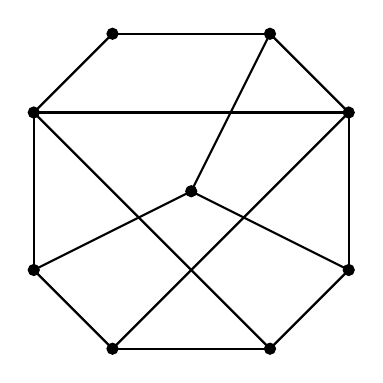
\begin{tikzpicture}
        \draw[black, thick] (0,1) -- (1,0);
        \draw[black, thick] (0,1) -- (2,2);
        \draw[black, thick] (3,4) -- (2,2);
        \draw[black, thick] (3,4) -- (1,4);
        \draw[black, thick] (0,3) -- (1,4);
        \draw[black, thick] (4,3) -- (3,4);
        \draw[black, thick] (1,0) -- (4,3);
        \draw[black, thick] (1,0) -- (3,0);
        \draw[black, thick] (3,0) -- (4,1);
        \draw[black, thick] (3,0) -- (0,3);
        \draw[black, thick] (2,2) -- (4,1);
        \draw[black, thick] (0,1) -- (0,3);
        \draw[black, thick] (4,1) -- (4,3);
        \draw[black, thick] (0,3) -- (4,3);

        \filldraw[black] (1,0) circle (2pt);
        \filldraw[black] (0,1) circle (2pt);
        \filldraw[black] (3,0) circle (2pt);
        \filldraw[black] (4,1) circle (2pt);
        \filldraw[black] (2,2) circle (2pt);
        \filldraw[black] (0,3) circle (2pt);
        \filldraw[black] (4,3) circle (2pt);
        \filldraw[black] (1,4) circle (2pt);
        \filldraw[black] (3,4) circle (2pt);
    \end{tikzpicture}
    \caption{Nonplanar graph G}

\end{figure}

\begin{figure}[h]
    \centering
    \label{fig:G1}
    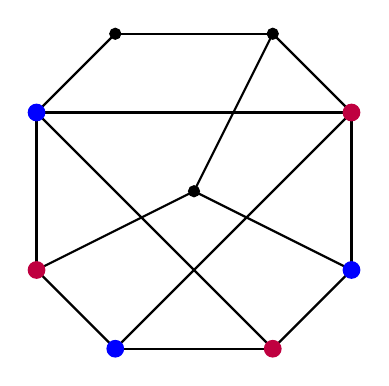
\begin{tikzpicture}
        \draw[black, thick] (0,1) -- (1,0);
        \draw[black, thick] (0,1) -- (2,2);
        \draw[black, thick] (3,4) -- (2,2);
        \draw[black, thick] (3,4) -- (1,4);
        \draw[black, thick] (0,3) -- (1,4);
        \draw[black, thick] (4,3) -- (3,4);
        \draw[black, thick] (1,0) -- (4,3);
        \draw[black, thick] (1,0) -- (3,0);
        \draw[black, thick] (3,0) -- (4,1);
        \draw[black, thick] (3,0) -- (0,3);
        \draw[black, thick] (2,2) -- (4,1);
        \draw[black, thick] (0,1) -- (0,3);
        \draw[black, thick] (4,1) -- (4,3);
        \draw[black, thick] (0,3) -- (4,3);

        \filldraw[blue] (1,0) circle (3pt);
        \filldraw[purple] (0,1) circle (3pt);
        \filldraw[purple] (3,0) circle (3pt);
        \filldraw[blue] (4,1) circle (3pt);
        \filldraw[black] (2,2) circle (2pt);
        \filldraw[blue] (0,3) circle (3pt);
        \filldraw[purple] (4,3) circle (3pt);
        \filldraw[black] (1,4) circle (2pt);
        \filldraw[black] (3,4) circle (2pt);

    \end{tikzpicture}
    \caption{Nonplanar graph G}
\end{figure}

\begin{center}
    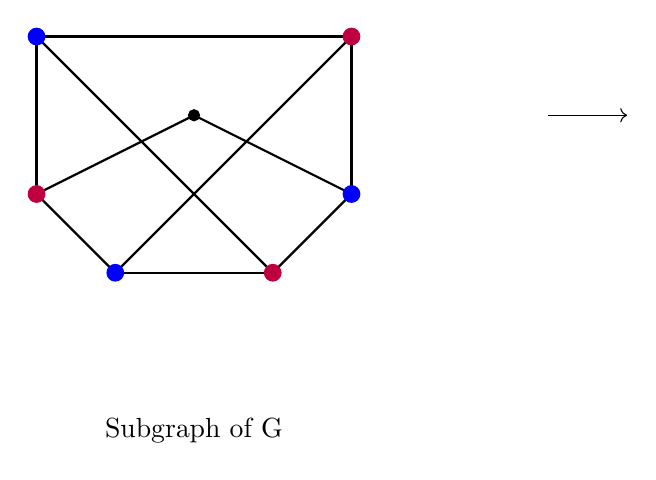
\begin{tikzpicture}
        \draw[black, thick] (0,1) -- (1,0);
        \draw[black, thick] (1,0) -- (4,3);
        \draw[black, thick] (1,0) -- (3,0);
        \draw[black, thick] (3,0) -- (4,1);
        \draw[black, thick] (3,0) -- (0,3);
        \draw[black, thick] (0,1) -- (0,3);
        \draw[black, thick] (4,1) -- (4,3);
        \draw[black, thick] (0,3) -- (4,3);
        \draw[black, thick] (0,1) -- (2,2);
        \draw[black, thick] (2,2) -- (4,1);
        \filldraw[blue] (1,0) circle (3pt);
        \filldraw[purple] (0,1) circle (3pt);
        \filldraw[purple] (3,0) circle (3pt);
        \filldraw[blue] (4,1) circle (3pt);
        \filldraw[blue] (0,3) circle (3pt);
        \filldraw[purple] (4,3) circle (3pt);
        \filldraw[black] (2,2) circle (2pt);
        \draw [-{To}] (6.5, 2) to (7.5, 2);
        \node at (2,-2,0) {Subgraph of G};
    \end{tikzpicture}
    \hspace{2cm}
    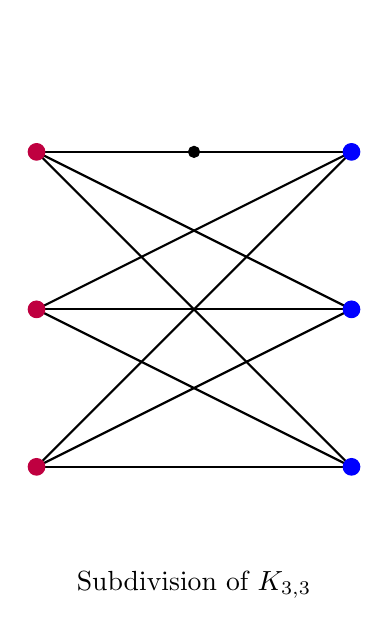
\begin{tikzpicture}
        \draw[black, thick] (8,-0.5) -- (12,-0.5);
        \draw[black, thick] (8,-0.5) -- (12,1.5);
        \draw[black, thick] (8,-0.5) -- (12,3.5);
        \draw[black, thick] (8,1.5) -- (12,-0.5);
        \draw[black, thick] (8,1.5) -- (12,1.5);
        \draw[black, thick] (8,1.5) -- (12,3.5);
        \draw[black, thick] (8,3.5) -- (12,-0.5);
        \draw[black, thick] (8,3.5) -- (12,1.5);
        \draw[black, thick] (8,3.5) -- (12,3.5);
        \filldraw[white] (10,5) circle (2pt);
        \filldraw[black] (10,3.5) circle (2pt);
        \filldraw[blue] (12,-0.5) circle (3pt);
        \filldraw[purple] (8,-0.5) circle (3pt);
        \filldraw[blue] (12,1.5) circle (3pt);
        \filldraw[purple] (8,1.5) circle (3pt);
        \filldraw[blue] (12,3.5) circle (3pt);
        \filldraw[purple] (8,3.5) circle (3pt);
        \node at (10,-2,0) {Subdivision of $K_{3,3}$};
    \end{tikzpicture}
\end{center}

\section{Preliminaries}

\subsection{Planar Graphs and their Properties}

\begin{definition}[Planarity]
    A graph is planar if some embedding of it onto the plane has no edge intersections.
\end{definition}

\begin{center}
    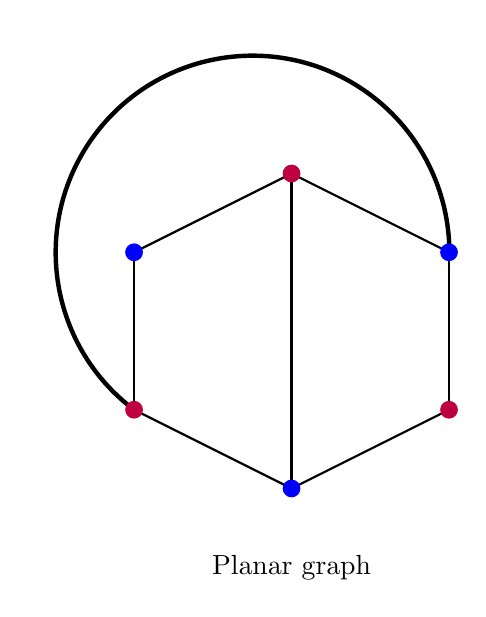
\begin{tikzpicture}
        \draw[black, thick] (0,1) -- (2,0);
        \draw[black, thick] (2,0) -- (4,1);
        \draw[black, thick] (4,1) -- (4,3);
        \draw[black, thick] (4,3) -- (2,4);
        \draw[black, thick] (2,0) -- (2,4);
        \draw[black, thick] (2,4) -- (0,3);
        \draw[black, thick] (0,3) -- (0,1);
        \draw[ultra thick] (0,1) arc (233:0:2.5);
        \filldraw[purple] (0,1) circle (3pt);
        \filldraw[purple] (4,1) circle (3pt);
        \filldraw[purple] (2,4) circle (3pt);
        \filldraw[blue] (0,3) circle (3pt);
        \filldraw[blue] (4,3) circle (3pt);
        \filldraw[blue] (2,0) circle (3pt);
        \node at (2,-1,0) {Planar graph};
    \end{tikzpicture}
    \hspace{2cm}
    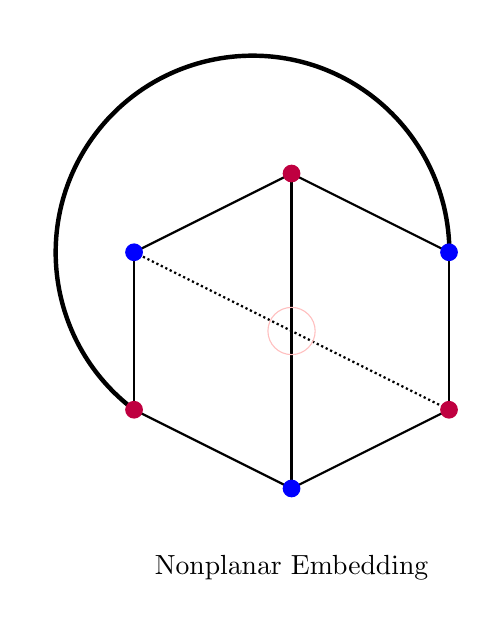
\begin{tikzpicture}
        \draw[black, thick] (0,1) -- (2,0);
        \draw[black, thick] (2,0) -- (4,1);
        \draw[black, thick] (4,1) -- (4,3);
        \draw[black, thick] (4,3) -- (2,4);
        \draw[black, thick] (2,0) -- (2,4);
        \draw[black, thick] (2,4) -- (0,3);
        \draw[black, thick] (0,3) -- (0,1);
        \draw[densely dotted, black, thick] (0,3) -- (4,1);
        \draw[ultra thick] (0,1) arc (233:0:2.5);
        \filldraw[purple] (0,1) circle (3pt);
        \filldraw[purple] (4,1) circle (3pt);
        \filldraw[purple] (2,4) circle (3pt);
        \filldraw[blue] (0,3) circle (3pt);
        \filldraw[blue] (4,3) circle (3pt);
        \filldraw[blue] (2,0) circle (3pt);
        \draw[pink] (2,2) circle (0.3);
        \node at (2,-1,0) {Nonplanar Embedding};
    \end{tikzpicture}
\end{center}

\subsection{Define $K_5$ and $K_{3,3}$}

\begin{center}
    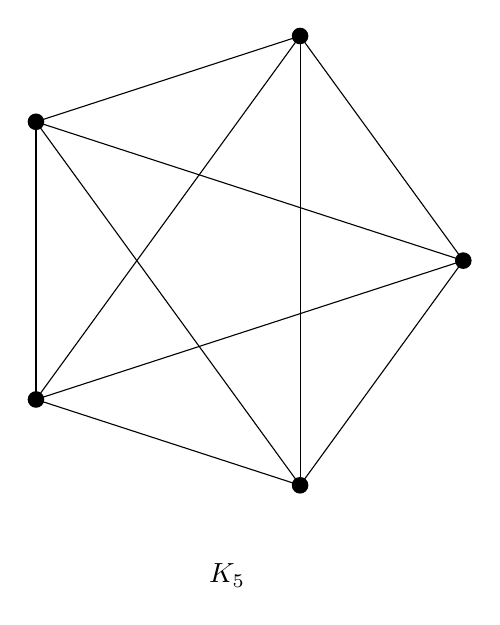
\begin{tikzpicture}
        \foreach \i in {1, 2, 3, 4, 5}
        \fill[black] (\i*360/5:3) coordinate (5\i) circle(3 pt)
        \ifnum \i>1 foreach \j in {\i,...,1}{(5\i) edge (5\j)} \fi;

        \node at (0,-4,0) {$K_5$};
    \end{tikzpicture}
    \hspace{2cm}
    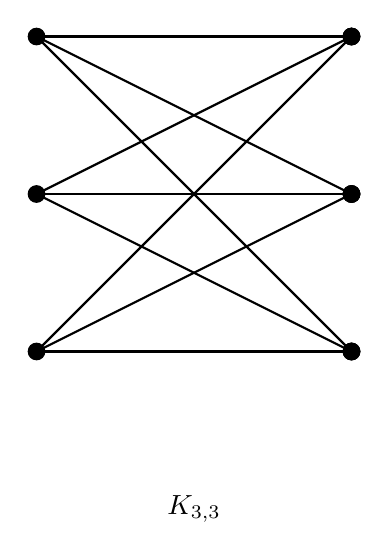
\begin{tikzpicture}
        \foreach \x/\y in {0/1, 0/3, 0/5} {
                \filldraw[black] (\x,\y) circle (3pt);
                \foreach \z/\t in {4/1, 4/3, 4/5} {
                        \filldraw[black] (\z,\t) circle (3pt);
                        \draw[black, thick] (\x,\y) -- (\z,\t);
                    }
            }
        \node at (2,-1,0) {$K_{3,3}$};
    \end{tikzpicture}
\end{center}

\subsection{Subgraph and Subdivision}
\begin{definition}
    Subgraphs are subsets of vertices and egdes of some original graphs
\end{definition}
\begin{center}
    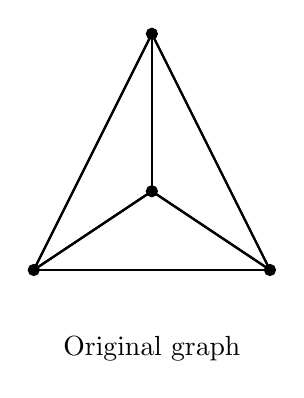
\begin{tikzpicture}
        \foreach \x/\y in {0/0, 1.5/1, 3/0, 1.5/3} {
                \filldraw[black] (\x,\y) circle (2pt);
                \foreach \z/\t in {0/0, 1.5/1, 3/0, 1.5/3} {
                        \draw[black, thick] (\x,\y) -- (\z,\t);
                    }
            }
        \node at (1.5,-1,0) {Original graph};
    \end{tikzpicture}
\end{center}

\begin{center}
    \begin{tikzpicture}
        \filldraw[black] (0,0) circle (2pt);
        \filldraw[black] (1.5,3) circle (2pt);
        \filldraw[black] (3,0) circle (2pt);
        \draw[black, thick] (0,0) -- (1.5,3);

        \filldraw[black] (7,0) circle (2pt);
        \filldraw[black] (8.5,3) circle (2pt);
        \filldraw[black] (10,0) circle (2pt);
        \draw[black, thick] (7,0) -- (8.5,3);
        \draw[black, thick] (10,0) -- (8.5,3);
        \draw[black, thick] (10,0) -- (7,0);

        \filldraw[black] (14,0) circle (2pt);
        \filldraw[black] (15.5,3) circle (2pt);
        \filldraw[black] (17,0) circle (2pt);
        \filldraw[black] (15.5,1) circle (2pt);
        \draw[black, thick] (14,0) -- (15.5,3);
        \draw[black, thick] (14,0) -- (15.5,1);
        \draw[black, thick] (15.5,3) -- (15.5,1);
        \draw[black, thick] (17,0) -- (15.5,3);
        \node at (8.5, -1, 0) {3 Subgraphs};
    \end{tikzpicture}
\end{center}

\begin{corollary}
    If graph is planar then all subgraphs are planar
\end{corollary}

\begin{proof}
    Contradiction
\end{proof}

\begin{definition}
    Subdivisions are obtained by replacing an edge with 2 edges connected by a new vertex
\end{definition}

\begin{center}
    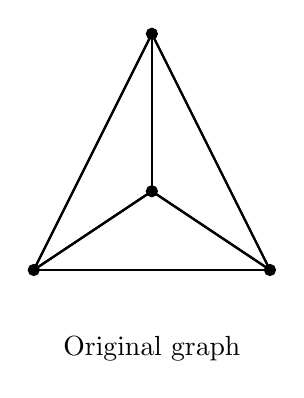
\begin{tikzpicture}
        \foreach \x/\y in {0/0, 1.5/1, 3/0, 1.5/3} {
                \filldraw[black] (\x,\y) circle (2pt);
                \foreach \z/\t in {0/0, 1.5/1, 3/0, 1.5/3} {
                        \draw[black, thick] (\x,\y) -- (\z,\t);
                    }
            }
        \node at (1.5,-1,0) {Original graph};
    \end{tikzpicture}
    \hspace{2cm}
    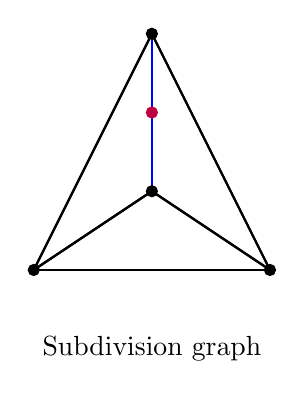
\begin{tikzpicture}
        \foreach \x/\y in {0/0, 1.5/1, 3/0, 1.5/3} {
                \foreach \z/\t in {0/0, 1.5/1, 3/0, 1.5/3} {
                        \draw[black, thick] (\x,\y) -- (\z,\t);
                    }
            }
        \node at (1.5,-1,0) {Subdivision graph};
        \draw[blue, thick] (1.5,1) -- (1.5,3);
        \filldraw[purple] (1.5,2) circle (2pt);
        \foreach \x/\y in {0/0, 1.5/1, 3/0, 1.5/3} {
                \filldraw[black] (\x,\y) circle (2pt);
            }
    \end{tikzpicture}
\end{center}

\begin{corollary}
    If some subdivision is planar then graph is planar
\end{corollary}
\begin{proof}
    Ai biết đâu.
\end{proof}
\begin{lemma}
    If graph is nonplanar then all subdivisions are nonplanar
\end{lemma}
\subsection{2-Connected Graphs and their Properties}
\begin{definition}
    A graph is 2-connected if it cannot be separated into two components by removing a single vertex
\end{definition}
\begin{center}
    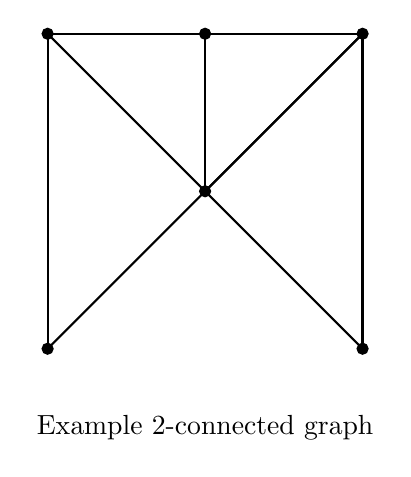
\begin{tikzpicture}
        \draw[black, thick] (0,0) -- (0,4);
        \draw[black, thick] (0,0) -- (4,4);
        \draw[black, thick] (4,0) -- (4,4);
        \draw[black, thick] (2,2) -- (4,4);
        \draw[black, thick] (2,2) -- (2,4);
        \draw[black, thick] (0,4) -- (4,4);
        \draw[black, thick] (0,4) -- (4,0);
        \foreach \x/\y in {0/0, 0/4, 2/2, 2/4, 4/0, 4/4} {
                \filldraw[black] (\x,\y) circle (2pt);
            }
        \node at (2,-1,0) {Example 2-connected graph};
    \end{tikzpicture}
    \hspace{2cm}
    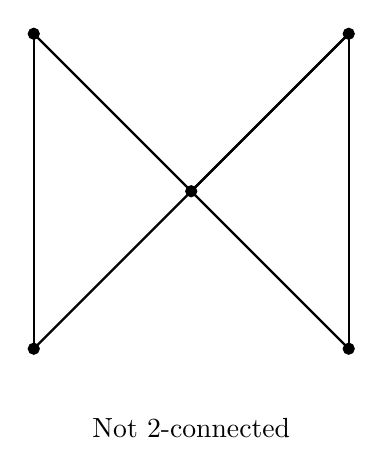
\begin{tikzpicture}
        \draw[black, thick] (0,0) -- (0,4);
        \draw[black, thick] (0,0) -- (4,4);
        \draw[black, thick] (4,0) -- (4,4);
        \draw[black, thick] (2,2) -- (4,4);
        \draw[black, thick] (0,4) -- (4,0);
        \foreach \x/\y in {0/0, 0/4, 2/2, 4/0, 4/4} {
                \filldraw[black] (\x,\y) circle (2pt);
            }
        \node at (2,-1,0) {Not 2-connected};
    \end{tikzpicture}
\end{center}
\begin{theorem}
    In a 2-connected graph, any pair of vertices is contained in a cycle
    \begin{proof}
        Quy nạp:

        Trường hợp cơ bản: $u$ kề $v$
        \begin{center}
            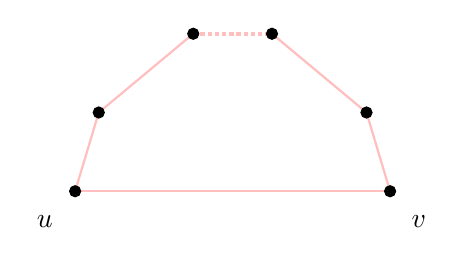
\begin{tikzpicture}
                \draw[pink, thick] (0,0) -- (0.3,1);
                \draw[pink, thick] (0.3,1) -- (1.5,2);
                \draw[densely dotted, pink, ultra thick] (1.5,2) -- (2.5,2);
                \draw[pink, thick] (2.5,2) -- (3.7,1);
                \draw[pink, thick] (3.7,1) -- (4,0);
                \draw[pink, thick] (0,0) -- (4,0);
                \node at (0,0,1) {$u$};
                \node at (4.75,0,1) {$v$};
                \filldraw[black] (0,0) circle (2pt);
                \filldraw[black] (0.3,1) circle (2pt);
                \filldraw[black] (1.5,2) circle (2pt);
                \filldraw[black] (2.5,2) circle (2pt);
                \filldraw[black] (3.7,1) circle (2pt);
                \filldraw[black] (4,0) circle (2pt);
            \end{tikzpicture}
        \end{center}
        Quy nạp: $u,v$ có khoảng cách $d+1$
        \begin{center}
            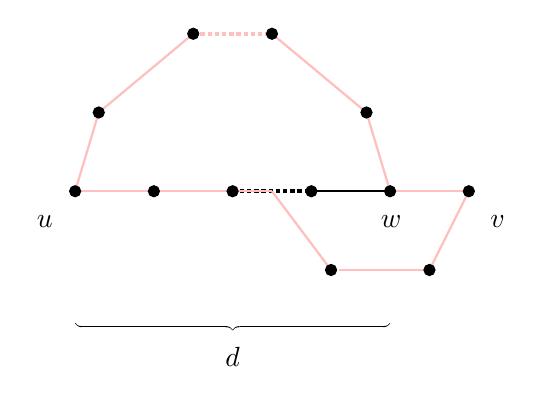
\begin{tikzpicture}
                \draw[pink, thick] (0,0) -- (0.3,1);
                \draw[pink, thick] (0.3,1) -- (1.5,2);
                \draw[densely dotted, pink, ultra thick] (1.5,2) -- (2.5,2);
                \draw[pink, thick] (2.5,2) -- (3.7,1);
                \draw[pink, thick] (3.7,1) -- (4,0);
                \draw[pink, thick] (0,0) -- (2,0);
                \draw[black, thick] (3,0) -- (4,0);
                \draw[pink, thick] (4,0) -- (5,0);
                \draw[densely dotted, black, ultra thick] (2,0) -- (3,0);
                \draw[pink, thick] (2.5,0) -- (3.25,-1);
                \draw[pink, thick] (3.35,-1) -- (4.5,-1);
                \draw[pink, thick] (5,0) -- (4.5,-1);
                \draw[pink, thick] (2,0) -- (2.5,0);


                \node at (0,0,1) {$u$};
                \node at (5.75,0,1) {$v$};
                \node at (4.4,0,1) {$w$};
                \filldraw[black] (0,0) circle (2pt);
                \filldraw[black] (0.3,1) circle (2pt);
                \filldraw[black] (1.5,2) circle (2pt);
                \filldraw[black] (2.5,2) circle (2pt);
                \filldraw[black] (3.7,1) circle (2pt);
                \filldraw[black] (1,0) circle (2pt);
                \filldraw[black] (2,0) circle (2pt);
                \filldraw[black] (3,0) circle (2pt);
                \filldraw[black] (4,0) circle (2pt);
                \filldraw[black] (5,0) circle (2pt);
                \filldraw[black] (3.25,-1) circle (2pt);
                \filldraw[black] (4.5,-1) circle (2pt);

                \draw [decorate, decoration = {calligraphic brace, mirror, raise=5pt}] (0,-1.5) --  (4,-1.5) node[pos=0.5,below=10pt,black]{$d$};
            \end{tikzpicture}
        \end{center}
    \end{proof}
\end{theorem}

\section{Graph Theory Background}
\begin{definition}[Fibration]
    A fibration is a mapping between two topological spaces that has the homotopy lifting property for every space $X$.
\end{definition}

\section{Proof the Theorem}
The first direction of \hyperref[thr:kuratowski]{Kuratowski's theorem} states: If graph $G$ contains a subdivision of $K_5$ or $K_{3,3}$ then $G$ is nonplanar

Subdivision of Nonplanar is Nonplanar

If a Subgraph is nonplanar then graph is nonplanar

If a subgraph of graph $G$ is a subdivision of nonplanar then $G$ is nonplanar
\begin{lemma}
    $K_{3,3}$ is nonplanar
\end{lemma}
\begin{proof}

    \begin{multicols}{3}
        $$V-E+F=2$$
        $$6-E+F=2$$
        $$6-9+F=2$$
        $$F=5$$

        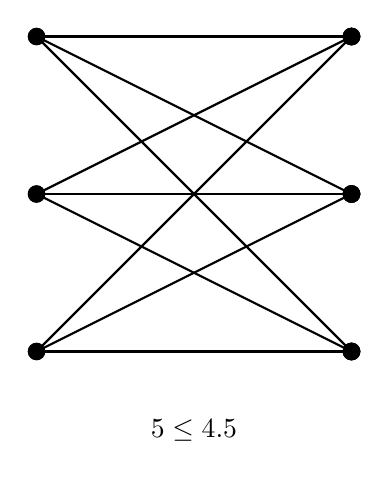
\begin{tikzpicture}
            \foreach \x/\y in {0/1, 0/3, 0/5} {
                    \filldraw[black] (\x,\y) circle (3pt);
                    \foreach \z/\t in {4/1, 4/3, 4/5} {
                            \filldraw[black] (\z,\t) circle (3pt);
                            \draw[black, thick] (\x,\y) -- (\z,\t);
                        }
                }
            \node at (2,0,0) {$5 \leq 4.5$};
        \end{tikzpicture}
        No 3 edge faces
        $$4F \leq 2E$$
        $$4F \leq 2 \times 9$$
        $$ F \leq 4.5$$
    \end{multicols}
\end{proof}

\begin{lemma}
    $K_5$ is nonplanar
\end{lemma}
\begin{proof}
    \begin{multicols}{3}
        $$V-E+F=2$$
        $$5-E+F=2$$
        $$5-10+F=2$$
        $$F=7$$
        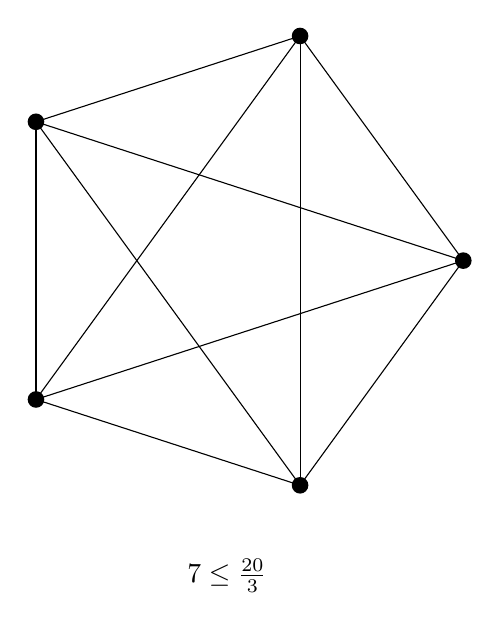
\begin{tikzpicture}
            \foreach \i in {1, 2, 3, 4, 5}
            \fill[black] (\i*360/5:3) coordinate (5\i) circle(3 pt)
            \ifnum \i>1 foreach \j in {\i,...,1}{(5\i) edge (5\j)} \fi;

            \node at (0,-4,0) {$7 \leq \frac{20}{3}$};
        \end{tikzpicture}

        $$3F \leq 2E$$
        $$3F \leq 2 \times 10$$
        $$F \leq \frac{20}{3}$$
    \end{multicols}
\end{proof}
\begin{recap}
    $K_5$ và $K_{3,3}$ are nonplanar

    $\Rightarrow$ All of their subdivisions are nonplanar

    $\Rightarrow$ If graph G contains a subdivision of $K_5$ or $K_{3,3}$ then G is nonplanar
\end{recap}

The second direction of \hyperref[thr:kuratowski]{Kuratowski's theorem} states: If graph $G$ is nonplanar then $G$ contains a subdivision of $K_5$ or $K_{3,3}$
\begin{proof}
    Assume there exist nonplanar graphs which have no subdivisions of $K_5$ or $K_{3,3}$ as subgraphs.

    Let G be the graph of this kind with the $fewest$ edges. Then removing any edge from $G$ gives a $planar$ graph

    \begin{enumerate}
        \item $G$ is 2-connected
              \begin{multicols}{2}
                  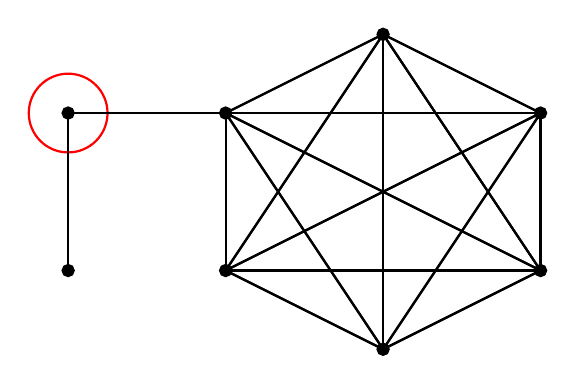
\begin{tikzpicture}
                      \draw[red, thick] (-2,3) circle (0.5);
                      \foreach \x/\y in {0/1, 2/0, 4/1, 0/3, 4/3, 2/4} {
                              \filldraw[black, thick] (\x,\y) circle (2pt);
                              \foreach \z/\t in {0/1, 2/0, 4/1, 0/3, 4/3, 2/4} {
                                      \draw[black, thick] (\x,\y) -- (\z,\t);
                                  }
                          }
                      \filldraw[black, thick] (-2,3) circle (2pt);
                      \filldraw[black, thick] (-2,1) circle (2pt);
                      \draw[black, thick] (-2,1) -- (-2,3);
                      \draw[black, thick] (-2,3) -- (0,3);

                  \end{tikzpicture}
              \end{multicols}
        \item $deg(v) \geq 3$ for all vertex $v$ in $G$

              Chứng minh phản chứng: assume some vertex $v \in G$ has $deg(v) \leq 2$

        \item for some $uv \in G$, $G - uv$ is 2-connected
    \end{enumerate}

\end{proof}

\begin{lemma}
    Given two line segments whose lengths are $a$ and $b$ respectively there
    is a real number $r$ such that $b=ra$.
\end{lemma}

\begin{proof}
    To prove it by contradiction try and assume that the statement is false,
    proceed from there and at some point you will arrive to a contradiction.
\end{proof}

\section*{Acknowledgement}
\addcontentsline{toc}{section}{Acknowledgement}
It is a pleasure to thank my mentor, Reid Harris, for his helpful guidance and advice. I would also like to thank Professor Babai for introducing me to graph theory and Professor May for organizing the REU.
\end{document}